\pagenumbering{arabic}
\section{实验一\ \ 系统调用、异常和外部中断}

% \subsection{实验环境}
% \textbf{硬件环境:}
% \begin{table}[htbp]
%     \centering
%     \begin{tabular}{cc}
%         \toprule
%         \bf CPU & Intel(R) Core(TM) i5-10210U \\
%         \bf RAM & 16.0 GB \\
%         \bottomrule
%     \end{tabular}
%     \caption{实验开发硬件环境}
%     \label{tab1-1}
% \end{table}

% \textbf{软件环境:}

% \begin{table}[htbp]
%     \centering
%     \begin{tabular}{cc}
%         \toprule
%         \bf VM & VMware 16.2.3 \\
%         \bf VM RAM & 8.0GB\\
%         \bf OS & Ubuntu 20.04 LTS \\
%         \bf Compiler & RISC-V Cross-compiler\\
%         \bf Simulator & Spike Simulator \\
%         \bottomrule
%     \end{tabular}
%     \caption{实验开发软件环境}
%     \label{tab1-1}
% \end{table}

\subsection{实验目的}
\begin{enumerate}
    \item 了解和掌握操作系统中系统调用机制的实现原理。
    \item 了解和掌握操作系统中异常(exception)的产生原理以及处理原则。
    \item 了解和掌握操作系统中外部中断(如时钟中断)的处理方法。
\end{enumerate}

\subsection{实验内容}

% \paragraph{lab1_1 系统调用} 找到并完成对do\_syscall的调用,获得预期输出结果。
% \paragraph{lab1_2 异常处理}
% 通过调用handle\_illegal\_instruction函数完成异常指令处理,阻止app\_illegal\_instruction的执行。
% \paragraph{lab1\_3 外部中断} 完成PKE操作系统内核未完成的时钟中断处理过程,使得它能够完整地处理时钟中断。




\paragraph{lab1_1 系统调用}
从user/app_helloworld.c文件中的两个函数调用printu和exit出发,对代码进行跟踪,找到系统调用过程中的缺失部分,并根据系统调用原理填补相应的代码,达到补全系统调用、实现相应功能的目的。

\begin{enumerate}
    \item 跟踪函数调用路径:\\
    printu\&exit(user/app_helloworld.c)\\ $\rightarrow$ printu\&exit(user/user_lib.c)\\ $\rightarrow$ do_user_call(user/user_lib.c)\\ $\rightarrow$  smode_trap_vector(kernel/strap_vector.S)\\
    $\rightarrow$ smode_trap_handler(kernel/strap.c)\\
    $\rightarrow$ handle_syscall(kernel/strap.c)(需要补全)\\
    $\rightarrow$ do_syscall(kernel/syscall.c)\\
    $\rightarrow$ sys_user_print\&sys_user_exit(kernel/syscall.c)
    \item 补全缺失的代码:handle_syscall函数尚未补全,需要增加对do_syscall的调用。需要注意的是调用时需要传入 tf->regs.a0 $\sim$ tf->regs.a7 八个寄存器的值作为参数,并将返回值存入 tf->regs.a0。补全的代码如下。
    \begin{cppcode}
static void handle_syscall(trapframe *tf) {
  tf->epc += 4;
  tf->regs.a0 = do_syscall(tf->regs.a0,tf->regs.a1,tf->regs.a2,tf->regs.a3,tf->regs.a4,
    tf->regs.a5,tf->regs.a6,tf->regs.a7);
}
\end{cppcode}
\end{enumerate}

\paragraph{lab1_2 异常处理}
分析CAUSE_ILLEGAL_INSTRUCTION异常处理模式和代理情况,跟踪异常处理路径并补全关键路径代码。
\begin{enumerate}
    \item 观察并分析kernel/machine/minit.c中的delegate_traps函数,发现PKE操作系统内核并没有将CAUSE_ILLEGAL_INSTRUCTION异常代理给S模式处理,仍在M模式下处理。
    \item 类似S模式的strap处理流程,M模式的trap处理入口在kernel/machine/mtrap_vector.S文件中,即mtrapvec过程。mtrapvec过程调用了handle_mtrap函数接管处理M模式下的trap。
    \item 在kernel/machine/mtrap.c中定义了handle_mtrap函数,发现case\ CAUSE_ILLEGAL_INSTRUCTION中的代码缺失,需要增加对handle_illegal_instruction函数的调用,补充的代码如下。
    \begin{cppcode}
void handle_mtrap() {
  uint64 mcause = read_csr(mcause);
  switch (mcause) {
    ......
    case CAUSE_ILLEGAL_INSTRUCTION:
      handle_illegal_instruction();
      break;
    ......
}
\end{cppcode}
\end{enumerate}

\paragraph{lab1_3 外部中断}
PKE内核代码在m_start函数(也就是机器模式的初始化函数)中新增了timerinit()函数(函数定义在kernel/machine/minit.c文件中),该函数设置了下一次timer触发的时间,还设置了MIE(Machine Interrupt Enable)寄存器中的MIE_MTIE位,即允许(模拟的)RISC-V机器在M模式处理timer中断。时钟中断的处理流程和lab1_2相仿,最终调用了机器模式下处理处理时钟中断的程序handle_timer,之后接力给S模式继续处理时钟中断。按照lab1_1的系统调用路径,在kernel/strap.c文件中的smode_trap_handler函数中增加了对CAUSE_MTIMER_S_TRAP的处理,处理函数为handle_mtimer_trap,需要根据实验需要补充完善handle_mtimer_trap函数,以达到正确处理时钟中断的目的。对handle_mtimer_trap函数需要进行以下完善:
\begin{enumerate}
    \item 对时钟中断计数器g_ticks进行加一操作。
    \item 对S模式的中断等待寄存器SIP(Supervisor Interrupt Pending)进行清除操作,即使用write_csr函数对SIP的SIP_SSIP位清零。
\end{enumerate}
函数中补充的内容如下。
\begin{cppcode}
void handle_mtimer_trap() {
    sprint("Ticks %d\n", g_ticks);
    g_ticks++;
    write_csr(sip, 0);
}
\end{cppcode}

\subsection{实验调试与测试结果}
\paragraph{lab1_1 系统调用} 系统调用实验的测试程序如下所示。
%图\ref{fig:lab1-1-testbench}
\begin{cppcode}
#include "user_lib.h"
int main(void) {
  printu("Hello world!\nHello wyz!\n");
  exit(0);
}
\end{cppcode}
% \begin{figure}[!htbp]
%     \centering
%     \includegraphics[width = 9cm]{figure/lab1_1_testbench.png}
%     \caption{lab1_1系统调用测试程序}
%     \label{fig:lab1-1-testbench}
% \end{figure}
编译运行测试程序,程序测试结果如图\ref{fig:lab1-1-testres}所示,程序打印出了"Hello world!"和"Hello wyz!"两行字符串,并正常退出,说明系统调用实验成功完成。
\begin{figure}[!htbp]
    \centering
    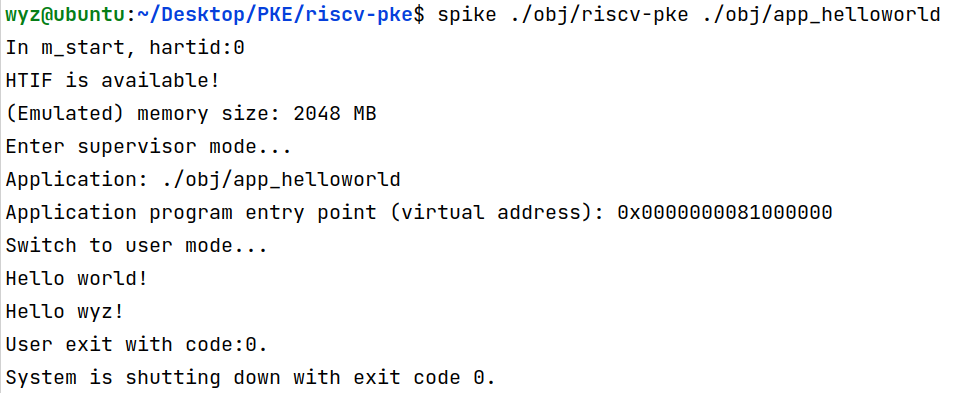
\includegraphics[width = 13cm]{figure/lab1_1_testresult.png}
    \caption{lab1_1系统调用测试结果}
    \label{fig:lab1-1-testres}
\end{figure}

\paragraph{lab1_2 异常处理}
异常处理实验的测试程序如下所示。
% 图\ref{fig:lab1-2-testbench}
\begin{cppcode}
#include "user_lib.h"
#include "util/types.h"
int main(void) {
  printu("Going to hack the system by running privilege instructions.\n");
  asm volatile("csrw sscratch, 0");
  exit(0);
}
\end{cppcode}
% \begin{figure}[!htbp]
%     \centering
%     \includegraphics[width = 12cm]{figure/lab1_2_testbench.png}
%     \caption{lab1_2异常处理测试程序}
%     \label{fig:lab1-2-testbench}
% \end{figure}
编译运行测试程序,程序测试结果如图\ref{fig:lab1-2-testres}所示,打印了异常指令提示字符串"Illegal instruction!
"并以"-1"作为退出码退出程序,说明异常处理实验成功完成。
\begin{figure}[!htbp]
    \centering
    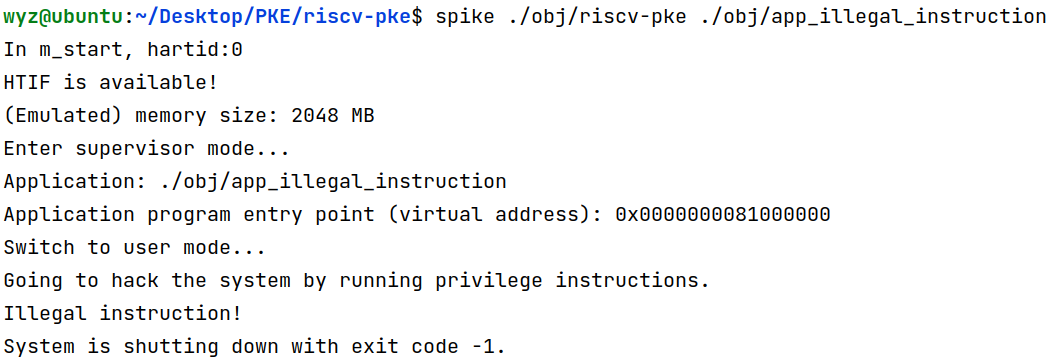
\includegraphics[width = 12cm]{figure/lab1_2_testresult.png}
    \caption{lab1_2异常处理测试结果}
    \label{fig:lab1-2-testres}
\end{figure}
\paragraph{lab1_3 外部中断} 
外部中断实验的测试程序如下所示,由于篇幅限制,测试程序设置为执行 $40000000$ 次循环,每 $10000000$ 次执行一次输出。
% 图\ref{fig:lab1-3-testbench}

\begin{cppcode}
#include "user_lib.h"
#include "util/types.h"

int main(void) {
  printu("Hello world!\n");
  int i;
  for (i = 0; i < 40000000; ++i) {
    if (i % 10000000 == 0) printu("wait %d\n", i);
  }
  exit(0);
}
\end{cppcode}
% \begin{figure}[!htbp]
%     \centering
%     \includegraphics[width = 10cm]{figure/lab1_3_testbench.png}
%     \caption{lab1_3外部中断测试程序}
%     \label{fig:lab1-3-testbench}
% \end{figure}
编译运行测试程序,程序测试结果如图\ref{fig:lab1-3-testres}所示,约每执行 10000000 次循环响应一次时钟中断,记录了时钟中断发生次数,并在程序运行结束后正常退出,说明外部中断处理实验成功完成。
\begin{figure}[!htbp]
    \centering
    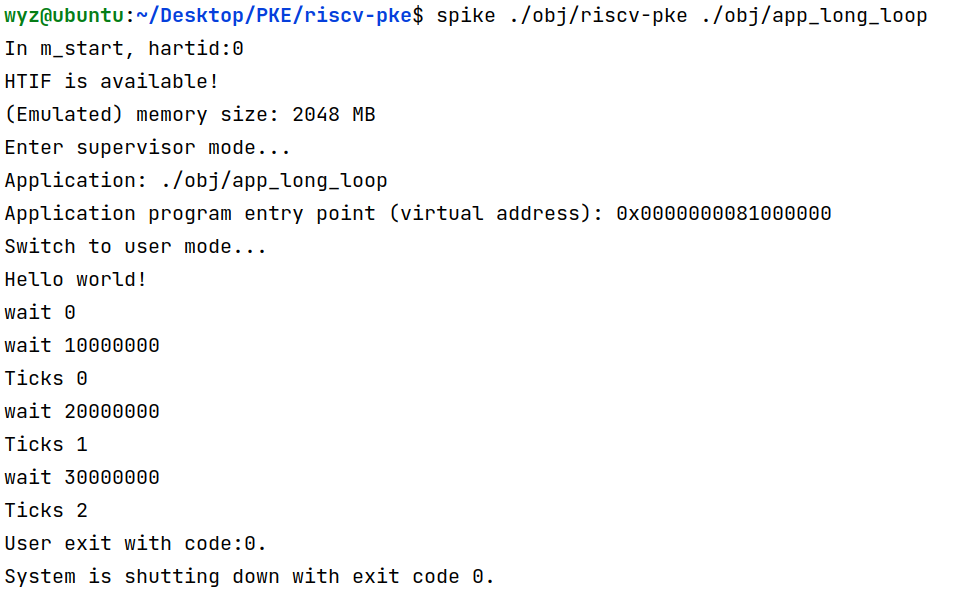
\includegraphics[width = 12cm]{figure/lab1_3_testresult.png}
    \caption{lab1_3外部中断测试结果}
    \label{fig:lab1-3-testres}
\end{figure}
\subsection{实验心得}
在此次实验中,我通过对PKE操作系统源码的阅读、跟踪与分析,了解并掌握了一个较为真实的操作系统中系统调用机制的实现原理、异常(exception)的产生原理和处理原则以及外部中断的处理方法。

在实验过程中,我通过对PKE操作系统S态和M态的trap处理机制的阅读、理解与补全,对多种特权级模式的权限以及不同特权级之间的切换有了更为清晰的认识;此外,我也进一步理解了系统调用、异常和外部中断这三个较为相似的概念之间的异同,掌握了它们的不同处理方法。

总之,虽然实验一的基础实验部分需要补全的代码量较少,但总体还是以阅读源码与理解原理为主,完成此次实验的收获还是颇为丰厚的。


